\documentclass[11pt]{article}
\usepackage[utf8]{inputenc}
\usepackage[T1]{fontenc}
\usepackage{amsmath}
\usepackage{amssymb}
\usepackage{multicol}
\usepackage{geometry}
\usepackage{tikz}
\usepackage{enumitem}
\usepackage{xcolor}
\usepackage{titlesec}

% Configurações de layout
\geometry{a4paper, left=1cm, right=1cm, top=0.5cm, bottom=1.2cm}
\setlength{\columnseprule}{0.4pt}

% Cores para títulos
\titleformat{\section}{\normalfont\Large\bfseries\color{blue}}{\thesection}{1em}{}
\titleformat{\subsection}{\normalfont\large\bfseries\color{red}}{\thesubsection}{1em}{}

% Reduz espaço antes e depois de seções e subseções
\titlespacing{\section}{0pt}{2ex}{1ex}
\titlespacing{\subsection}{0pt}{1.5ex}{0.5ex}

% Reduz espaço entre paragrafos 
\setlength{\parskip}{0pt}
\setlength{\parindent}{0pt}

% Reduz espaços em listas
\setlist{nosep, leftmargin=*}
\setlist[enumerate]{itemsep=0pt, topsep=0pt, partopsep=0pt, parsep=0pt}
\setlist[itemize]{itemsep=0pt, topsep=0pt, partopsep=0pt, parsep=0pt}

% Reduz espaço antes/depois de fórmulas
\setlength{\abovedisplayskip}{0pt}
\setlength{\belowdisplayskip}{0pt}
\setlength{\abovedisplayshortskip}{0pt}
\setlength{\belowdisplayshortskip}{0pt}

% Reduz espaço no multicols
\setlength{\multicolsep}{0pt}

\title{\textcolor{red}{Revisão: Medidas de Tendência Central \\
    Média, Mediana e Moda}}
\author{Professor: Jefferson}
\date{}

\begin{document}

\maketitle
\vspace{-1.0cm}

\begin{multicols}{2}

\section*{O que são Medidas de Tendência Central?}

São valores que representam um conjunto de dados, indicando um "ponto central" ou "típico" da distribuição.

\subsection*{Média Aritmética ($\bar{x}$)}

É a soma de todos os valores dividida pelo número total de elementos.

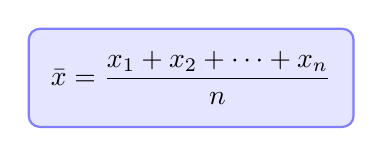
\begin{tikzpicture}
\node[rectangle, fill=blue!10, rounded corners, inner sep=8pt, draw=blue!50, thick] (box) {
$\displaystyle \bar{x} = \frac{x_1 + x_2 + \dots + x_n}{n}$
};
\end{tikzpicture}

\subsection*{Mediana (Md)}

É o valor central quando os dados estão ordenados.

\begin{itemize}
\item \textbf{n ímpar:} termo central
\item \textbf{n par:} média dos dois termos centrais
\end{itemize}

\subsection*{Moda (Mo)}

É o valor que aparece com maior frequência.

\begin{itemize}
\item \textbf{Unimodal:} uma moda
\item \textbf{Bimodal:} duas modas
\item \textbf{Amodal:} nenhuma moda
\end{itemize}

\section*{Exemplos}

\subsection*{Exemplo 1:}
Dados: 5, 7, 9, 11, 13

\[
\bar{x} = \frac{5+7+9+11+13}{5} = \frac{45}{5} = 9
\]
Mediana = 9 (termo central) \\
Moda = amodal

\subsection*{Exemplo 2:}
Dados: 4, 6, 6, 8, 10, 12

\[
\bar{x} = \frac{4+6+6+8+10+12}{6} = \frac{46}{6} \approx 7,67
\]
Mediana = $\frac{6+8}{2} = 7$ \\
Moda = 6

\section*{Exercícios Básicos}

\begin{enumerate}[leftmargin=*]

\item Calcule a média dos conjuntos:
\begin{enumerate}[label=\alph*)]
\item 10, 12, 14, 16, 18
\item 5, 8, 11, 14, 17, 20
\item 2, 4, 6, 8, 10, 12, 14
\item 15, 20, 25, 30, 35
\end{enumerate}

\item Determine a mediana:
\begin{enumerate}[label=\alph*)]
\item 3, 5, 7, 9, 11
\item 2, 4, 6, 8, 10, 12
\item 10, 15, 20, 25, 30, 35, 40
\item 1, 3, 5, 7, 9, 11, 13, 15
\end{enumerate}

\item Identifique a moda:
\begin{enumerate}[label=\alph*)]
\item 2, 3, 4, 4, 5, 6, 6, 6, 7
\item 10, 12, 12, 14, 14, 16, 18
\item 5, 5, 5, 8, 8, 10, 10, 10, 12
\item 1, 2, 3, 4, 5, 6
\end{enumerate}

\item Para o conjunto: 12, 15, 18, 21, 24, 27, 30
\begin{enumerate}[label=\alph*)]
\item Calcule a média
\item Determine a mediana
\item Identifique a moda
\end{enumerate}

\item Um aluno tirou as seguintes notas: 7,0; 8,5; 6,0; 9,0; 7,5. Qual sua média?

\item As idades de um grupo são: 12, 14, 13, 15, 12, 16, 14, 13, 12. Determine:
\begin{enumerate}[label=\alph*)]
\item Média
\item Mediana
\item Moda
\end{enumerate}

\end{enumerate}

\section*{Exercícios Intermediários}

\begin{enumerate}[leftmargin=*, start=7]

\item Uma empresa tem 5 funcionários com salários: R\$ 1800, R\$ 2000, R\$ 2200, R\$ 2500, R\$ 5000.
\begin{enumerate}[label=\alph*)]
\item Calcule a média salarial
\item Determine a mediana
\item Qual medida representa melhor o salário típico? Por quê?
\end{enumerate}

\item Em uma prova, as notas foram: 5, 6, 7, 8, 8, 9, 10, 10, 10.
\begin{enumerate}[label=\alph*)]
\item Qual a média?
\item Qual a mediana?
\item Qual a moda?
\end{enumerate}

\item Complete a tabela com as medidas:

\begin{center}
\begin{tabular}{|c|c|c|c|}
\hline
\textbf{Dados} & \textbf{Média} & \textbf{Mediana} & \textbf{Moda} \\
\hline
4, 8, 12, 16, 20 & & & \\
\hline
3, 5, 5, 7, 9, 11 & & & \\
\hline
10, 20, 30, 40, 50, 60 & & & \\
\hline
\end{tabular}
\end{center}

\item As temperaturas de uma semana: 22, 24, 23, 25, 24, 26, 24 (em °C).
\begin{enumerate}[label=\alph*)]
\item Qual a temperatura média?
\item Qual a temperatura mediana?
\item Qual a moda?
\end{enumerate}

\item Em uma pesquisa sobre número de irmãos:
\[
\begin{array}{c|c}
\text{Nº de irmãos} & \text{Frequência} \\
\hline
0 & 5 \\
1 & 8 \\
2 & 6 \\
3 & 3 \\
4 & 2 \\
\end{array}
\]
Calcule a média, mediana e moda.

\item Uma loja vendeu em 7 dias: 12, 15, 10, 18, 20, 15, 14 produtos.
\begin{enumerate}[label=\alph*)]
\item Quantidade média vendida
\item Quantidade mediana
\item Quantidade modal
\end{enumerate}

\end{enumerate}

\section*{Exercícios Avançados}

\begin{enumerate}[leftmargin=*, start=13]

\item Em uma turma, as notas foram:
\[
\begin{array}{c|c}
\text{Nota} & \text{Nº de alunos} \\
\hline
5 & 2 \\
6 & 4 \\
7 & 6 \\
8 & 5 \\
9 & 3 \\
10 & 2 \\
\end{array}
\]
\begin{enumerate}[label=\alph*)]
\item Calcule a média ponderada
\item Determine a mediana
\item Qual a moda?
\end{enumerate}

\item Três números têm média 15. Dois deles são 12 e 18. Qual é o terceiro número?

\item A média de 5 números é 20. Se retirarmos um número, a média dos 4 restantes é 18. Qual número foi retirado?

\item Em uma empresa, a média salarial é R\$ 2500. Se contratarmos um novo funcionário com salário R\$ 3000, a média passa para R\$ 2600. Quantos funcionários havia inicialmente?

\item Um conjunto de dados tem média 10 e mediana 12. Se adicionarmos o número 15 ao conjunto, o que podemos afirmar sobre a nova média e mediana?

\item (Desafio) Em uma classe, 60\% dos alunos são meninas. A média das notas das meninas é 8,0 e a média dos meninos é 6,0. Qual a média da turma toda?

\item Uma sequência de 5 números inteiros positivos tem mediana 8 e moda 10. Qual é a menor média possível?

\item Interpretação de gráfico:

\begin{center}
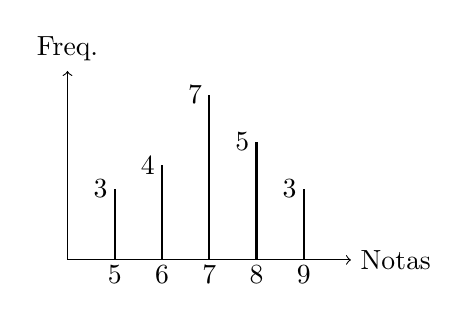
\begin{tikzpicture}[scale=0.6]
\draw[->] (0,0) -- (6,0) node[right] {Notas};
\draw[->] (0,0) -- (0,4) node[above] {Freq.};
\draw[thick] (1,0) -- (1,1.5);
\draw[thick] (2,0) -- (2,2);
\draw[thick] (3,0) -- (3,3.5);
\draw[thick] (4,0) -- (4,2.5);
\draw[thick] (5,0) -- (5,1.5);
\node at (1,-0.3) {5};
\node at (2,-0.3) {6};
\node at (3,-0.3) {7};
\node at (4,-0.3) {8};
\node at (5,-0.3) {9};
\node at (0.7,1.5) {3};
\node at (1.7,2) {4};
\node at (2.7,3.5) {7};
\node at (3.7,2.5) {5};
\node at (4.7,1.5) {3};
\end{tikzpicture}
\end{center}

Determine a média, mediana e moda das notas representadas.

\item Complete as lacunas:

\begin{enumerate}[label=\alph*)]
\item A \_\_\_\_\_\_ é o valor que divide o conjunto em duas partes iguais.
\item Quando a média é maior que a mediana, a distribuição é \_\_\_\_\_\_ à direita.
\item A \_\_\_\_\_\_ é a medida mais afetada por valores extremos.
\end{enumerate}

\end{enumerate}

\end{multicols}

\end{document}
